\documentclass{article}
\usepackage[utf8]{inputenc}
\usepackage[document]{ragged2e}
\usepackage{algpseudocode}
\usepackage[]{algorithmicx}
\usepackage{amsmath}
\usepackage{amsthm}
\usepackage{amssymb}
\usepackage[]{listings}
\usepackage{graphicx}
\usepackage{hyperref}
\usepackage{flafter}
\usepackage{subfig}
\usepackage{dsfont}
\graphicspath{ {images/} }

\begin{document}

\begin{titlepage}
	\centering
	%
\includegraphics[width=0.15\textwidth]{IIIT-B_logo.jpg}\par\vspace{1cm}
	{\scshape\LARGE International Institute of Information Technology, Bangalore \par}
	\vspace{1cm}
	{\scshape\Large Project Strategy Document\par}
	{\Large  DS 707 Data Analytics\par}
	\vspace{1.5cm}
	{\huge\bfseries Clustering and Association \par}
	\vspace{2cm}
	{\Large\itshape Akanksha Dwivedi - MT2016006\par}
	{\Large\itshape Hitesha Mukherjee - MS2016007\par}
	{\Large\itshape Nayna Jain - MS2017003\par}
	{\Large\itshape Tarini Chandrashekhar - MT2016144\par}
	\vfill
	Instructors : \par
	Prof. Ramanathan Chandrashekhar
	\par
	Prof. Uttam Kumar

	\vfill
% Bottom of the page
	{\large \today\par}
\end{titlepage}

\newpage

\section{Introduction}
As with stock market, cryptocurrency is growing investment area for the daily traders and investors. Cryptocurrency is very new and still stabilizing. Because of which it is very volatile in nature and might get affected by different factors. In such an environment it is very difficult to predict the price movement of cryptocurrencies.

Since the trend and investment point of view is similar to stock market, the established techniques used in stock market prediction are considered for cryptocurrency.

[1][2] refers to the papers which shows how clustering is used in the process of stock price prediction.

Clustering is the process of grouping of set of data objects into multiple groups or clusters so that objects within a cluster have high similarity, but are very dissimilar to objects in other clusters. It is called as unsupervised learning because the class label information is not present. Clustering is used for automatic classification, data segmentation and outlier detection.


We have applied similar techniques from [1] for the cryptocurrency forecasting.
[1] discusses three steps for forecasting which are:
\begin{itemize}
	\item Normalizing the data
	\item K-means clustering of the normalized data to identify the outliers
	\item ARIMA for forecasting on clustered data.
\end{itemize}

Thus, we see how clustering is applied to remove the outliers from the clusters.


\section{Clustering Techniques}
\subsubsection{K-Means Clustering}

It is a centroid based partitioning technique that uses the centroid of a cluster, Ci to represent the cluster. Conceptually, the centroid of a cluster is its center point. This algorithm requires to specify the number of clusters (k) beforehand. This method is not guaranteed to converge to the global optimum and often terminates to a local optimum.

We have applied this algorithm on Open/High attributes of the daily prices. And with some experimentation, of taking no of clusters values from 3, 4, 5, we found that between 4 and 5 here is not much difference. And so we decided to take the k value as 4. We attempt to identify the outliers based on these attributes.

\begin{figure}
	\centering
	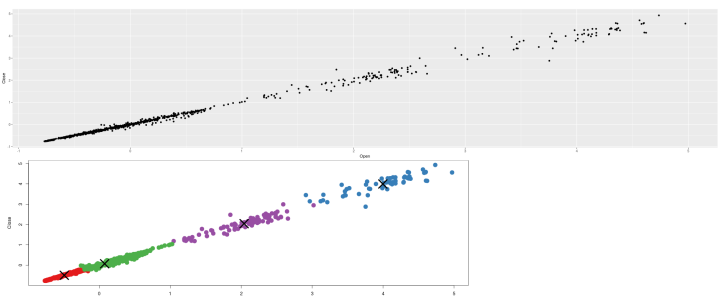
\includegraphics[width=\linewidth]{images/KMeansClustering}
	\caption{Before and After K Means Clustering}
	\label{fig:kmeansclustering}
\end{figure}



\begin{thebibliography}{widestlabel}
	
\bibitem{1}
STOCK MARKET TRENDS USING CLUSTER ANALYSIS AND ARIMA MODEL by Joyti Badge, Published in stock Market Trends
Asian-African Journal using of Economics Cluster Analysis
and Econometrics, and ARIMA Model Vol. 13, No. 2, 2013: 303-308

\bibitem{2}
ANALYSIS OF NIFTY FIFTY STOCKS BASED ON K-MEANS CLUSTERING TECHNIQUE FOR STOCK MARKET PREDICTION Dr. T.Chitra kalarani* and S.Indrakala**

\bibitem{3}
Book named "Data Mining Concepts and Techniques", Jiawei Han, Micheline Kamber, Jian Pei

\end{thebibliography}

\end{document}